\documentclass{report}
\usepackage{graphicx} % Required for inserting images
\usepackage[italian]{babel}
\usepackage{tikz}
\usepackage{hyperref}
\usepackage{amsmath}
\usepackage{xcolor}

\definecolor{darkgreen}{rgb}{0.0, 0.5, 0.0}


\title{Protezione di Macrodata e Microdata}
\date{Parte II}

\begin{document}

\maketitle

\tableofcontents
\newpage

Spesso il rilascio di dati statistici può inferire a dati non 
intesi per il rilascio.

La rivelazione può avvenire:
\begin{itemize}
    \item con i soli dati rilasciati
    \item dalla combinazione dei dati rilasciati con informazioni disponibili al pubblico
    \item dalla combinazione dei dati rilasciati con informazioni provenienti da altre fonti 
\end{itemize}


\chapter{Statistical DBMS}
Un \textbf{DBMS statistico} è un DBMS che offre accesso a statistiche 
su gruppi di invidui. Non deve rivelare nessuna informazione su nessun
individuo in particolare.

Le informazioni confidenziali possono essere dedotte:
\begin{itemize}
    \item combinando i risultati di statistiche differenti
    \item combinando i risultati delle statistiche con conoscenza esterna
\end{itemize} 

\begin{figure}[ht]
    \centering
    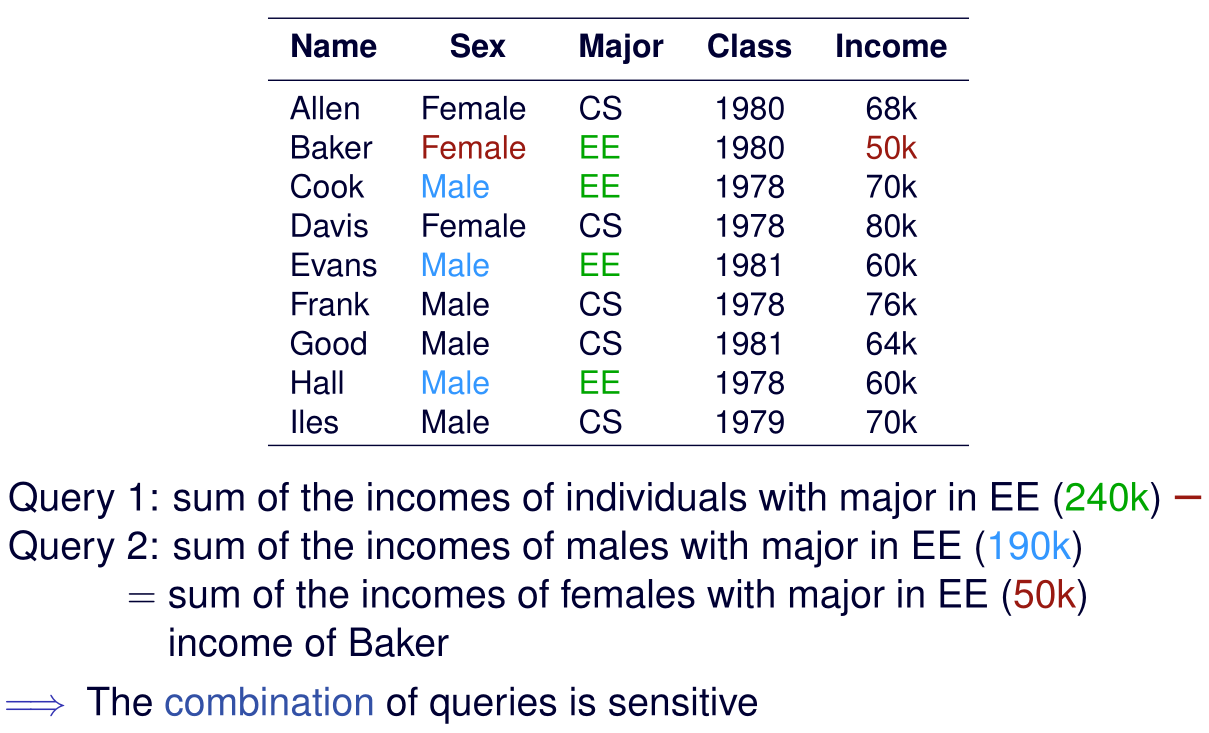
\includegraphics[width=1\linewidth]{images/stat-dbms.png}
\end{figure}

Una \textit{sensitive query} è una query che può provocare una \textit{disclosure}, ovvero la rivelazione di informazioni sensibili su un individuo.
Le query, prese singolarmente, potrebbero non essere sensibili, ovvero non rivelare informazioni confidenziali. 
Tuttavia, un insieme di query considerate nel loro complesso può diventare sensibile. Questo fenomeno è noto come \textit{\textbf{collusione}}. 
Attraverso la collusione, le informazioni aggregate da query non sensibili possono portare alla deduzione di dati privati o confidenziali.

Questa è la ragione per cui mi serve il controllo basato sulla 
storia: devo tenere traccia di quello che mi chiedi e della 
conoscenza che hai, e quindi di cosa puoi inferire.

\chapter{Protezione di Macrodata: tabelle di conteggio o frequenze}

La protezione di questo tipo di tabelle si divide in tre fasi:
\begin{enumerate}
    \item Sampling
    \item Identificazione delle celle sensibili
    \begin{itemize}
        \item special rules 
        \item threshold rules 
    \end{itemize}
    \item Protezione delle celle sensibili
    \begin{itemize}
        \item table restructuring
        \item soppressione 
        \item rounding 
        \item confidentiality edit
    \end{itemize}
\end{enumerate}

\section{Sampling}
Stabilisco un campione della popolazione totale (che sia rappresentativo, senza bias, \dots) 
e faccio la statistica su tale campione.

Prima di aggregare i dati, i singoli valori vengono moltiplicati per un peso (\textit{sampling weight});
in questo modo viene mantenuta la correlazione statistica dei dati ma introducendo del rumore (se i pesi non vengono pubblicati), rendendo 
più difficile identificare i dati dei singoli rispondenti dai valori pubblicati.

\section{Identificazione delle celle sensibili}

\subsection{Regole Speciali}
Le regole speciali definiscono il livello di dettaglio oltre il quale non è consentito
rilasciare dati.

Vengono chiamate in questo modo perché dipendono dall'agenzia e dal tipo di tabella
(dominio di applicazione).

Per soddisfare le regole speciali si può utilizzare:
\begin{itemize}
    \item table restructuring
    \item category combination
\end{itemize}

\subsection{Threshold rules}
Una cella viene considerata sensibile se il numero di rispondenti è inferiore 
a un certo numero specificato. 

\section{Protezione delle celle sensibili}
\subsection{Table Restructuring}
La tabella viene ristrutturata e righe o colonne vengono 
combinate (\textit{rolling-up categories}).

\subsection{Soppressione delle celle}
È una delle tecniche di protezione più usata. La sola soppressione delle celle 
sensibili non è sufficiente (\textbf{soppressione primaria}): è necessaria una seconda soppressione (\textbf{soppressione complementare})
per ogni riga e colonna in cui viene soppressa una cella sensibile, altrimenti 
il valore della cella sensibile potrebbe essere calcolabile dal totale marginale.

La scelta delle celle per la soppressione complementare è un problema difficile; possono essere
utilizzati modelli di programmazione lineare in cui l'obiettivo è 
massimizzare o minimizzare una funzione obiettivo, soggetta a dei vincoli:
\begin{itemize}
    \item la funzione obiettivo potrebbe essere la minimizzazione delle celle soppresse o la massimizzazione della protezione dei dati 
    \item i vincoli possono essere dei requisiti di riservatezza, come il numero minimo di celle da sopprimere o la necessità di mantenere la validità statistica dei dati 
\end{itemize}

\subsection{Rounding}
Per ridurre la perdita di dati dovuta alla soppressione, si utilizza il \textit{rounding} 
dei valori a un multiplo della soglia di sensibilità. Esistono due approcci possibili:
\begin{itemize}
    \item \textbf{Random:} viene scelto in maniera casuale se arrotondare i valori per eccesso o per difetto 
    \begin{itemize}
        \item la conseguenza è che la somma dei valori in una riga o in una colonna 
        potrebbe differire dai totali marginali
    \end{itemize}
    \item \textbf{Controllato:} garantisce che la somma delle righe e colonne siano uguali 
    ai totali marginali
    \begin{itemize}
        \item \textbf{\textcolor{darkgreen}{Vantaggi:}} garantisce che i dati pubbliati siano coerenti con i totali marginali
        \item \textbf{\textcolor{red}{Svantaggi:}} richiede l'uso di programmi informatici specializzati per il calcolo delle soluzioni di arrotondamento; non sempre potrebbero esistere soluzioni
    \end{itemize}
\end{itemize}

\subsubsection{Nota}
Tutti i valori delle celle devono essere multiplo del valore di \textit{sensitivity threshold}; è 
fondamentale per mantenere la riservatezza e l'integrità dei dati.


\subsection{Confidentiality Edit}
La \textit{confidentiality edit} viene applicata attraverso un processo di switching:
\begin{enumerate}
    \item si prende un campione di record dal file di microdati
    \item si trova una corrispondenza per tali record in una popolazione contenente altri record (ad esempio un'altra regione geografica)
    \item si scambiano tutti gli attributi sui record che corrispondono
\end{enumerate}

\subsubsection{Nota}
Si opera non sulla statistica ma sui dati su cui viene prodotta tale statistica; la 
protezione è garantita dal fatto che sto introducendo del rumore nei dati.

\chapter{Protezione di Macrodata: tabelle di magnitudo}
È probabile che la distribuzione dei valori riportati nelle tabelle di magnitudo sia
asimmetrica (\textit{skewed}); le tecniche di limitazione di disclosure si concentrano 
sulla prevenzione della stima precisa dei valori per gli outlier.

\section{Identificazione delle celle sensibili}
Per identificare le celle sensibili si utilizzano le \textit{regole di soppressione},
che cercano di verificare
se è sufficientemente difficile per un rispondente stimare il valore di un altro 
rispondente in modo troppo preciso.

Queste regole vengono definite \textbf{regole di soppressione primaria}.

\subsection{\textit{p-percent} rule}
Questa regola stabilisce una soglia percentuale al di sotto della quale i valori 
delle celle sono considerati sensibili.; verifica se è sufficientemente difficile per 
un rispondente stimare troppo accuratamente il contributo di un rispondente.

\begin{itemize}
    \item Una cella è considerata \textbf{sensibile} se le stime superiori e inferiori per 
    il valore del rispondente sono più vicine al valore riportato di una percentuale 
    stabilita $p$. (è possibile inferire sotto a un certo intervallo di incertezza il dato)
    \item Formalmente, una cella è considerata protetta se:
    \[
    \sum_{i=c+2}^{N} x_i \geq \frac{p}{100} x_1
    \]
    dove:
    \begin{itemize}
        \item \( x_1, x_2, \ldots, x_N \): valori dei rispondenti in ordine decrescente,
        \item \( c \): dimensione di una coalizione di rispondenti interessati a stimare \( x_1 \) (\textit{collusione}).
        \item il valore più grande \( x_1 \) è il più esposto (\textit{outlier}).
    \end{itemize}
\end{itemize}

\subsubsection{Esempio}
\begin{figure}[ht]
    \centering
    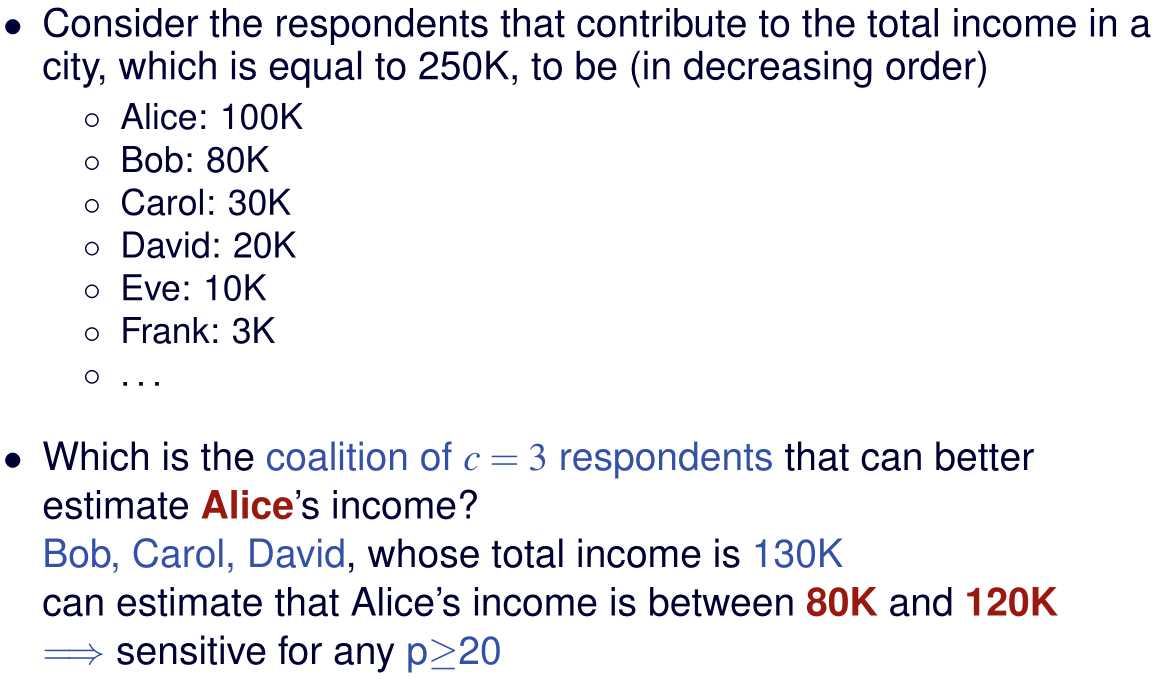
\includegraphics[width=1\linewidth]{images/p-perc.png}
\end{figure}

\subsection{\textit{pq} rule}
Possiamo definire questa regola come un affiniamento della regola precedente, che introduce 
la conoscenza pregressa con il valore $q$: rappresenta quanto accuratamente i rispondenti 
possono stimare il valore di un altro rispondente prima che i dati vengano pubblicati ($p<q<100$).

\begin{itemize}
    \item $q$ indica l'errore nella stima prima della pubblicazione 
    \item Formalmente, una cella è considerata protetta se:
    \[
    \frac{q}{100} \sum_{i=c+2}^{N} x_i \geq \frac{p}{100} x_1
    \]
    dove:
    \begin{itemize}
        \item \( x_1, x_2, \ldots, x_N \): valori dei rispondenti in ordine decrescente,
        \item \( c \): dimensione di una coalizione di rispondenti interessati a stimare \( x_1 \) (\textit{collusione}).
        \item il valore più grande \( x_1 \) è il più esposto (\textit{outlier}).
        \item la \textit{pq rule} si riduce alla \textit{p-percent rule} quando \( q = 100 \) (cioè, nessuna capacità di stima).
    \end{itemize}
\end{itemize}

\subsection{\textit{(n,k)} rule}
Questa regola stabilisce che, indipendentemente dal numero di rispondenti in una cella, 
se un numero ridotto ($\leq n$) di questi rispondenti contribuisce a una grande percentuale 
($\geq k$) del valore totale della cella, allora la cella viene considerata 
sensibile (spesso si usa $n=1$ o $n=2$).

\subsubsection{Regola intuitiva}
Se una cella è dominata da un solo rispondente, il totale pubblicato rappresenta 
una stima superiore per il suo valore.

\subsubsection{Esempio}
$(2, 70) \rightarrow $ sensibile se $\leq 2$ rispondenti fanno il $\geq 70$\% del totale.


\section{Protezione delle celle sensibili}
Una volta identificate le celle sensibili, ci sono due opzioni:
\begin{itemize}
    \item \textbf{ristrutturare la tabella e combinare le celle} fino a quando non 
    rimangono più celle sensibili
    \item \textbf{soppressione} delle celle sensibili
\end{itemize}

\subsubsection{Soppressione secondaria}
È necessario selezionare altre celle non sensibili da sopprimere, per garantire che i 
dati nelle celle sensibili non possano essere stimati con troppa accuratezza.

\noindent Le celle sensibili potrebbero essere divulgate a causa del fatto che:
\begin{itemize}
    \item le unioni delle celle soppresse possono essere sensibili secondo la regola di sensibilità adottata,
    \item le equazioni delle righe e delle colonne rappresentate dalla tabella pubblicata possono essere risolte, e il valore per una cella soppressa stimato con troppa accuratezza.
\end{itemize}

\newpage
\section{Verifica dei risultati}
\subsection{Audit}
L'audit è una fase di verifica in cui controllo che tutto sia protetto.

\noindent Se i totali vengono pubblicati, la somma delle celle soppresse può essere 
derivata. È necessario applicare la regola di sensibilità a queste somme per garantire
che non siano sensibili:
\begin{itemize}
    \item le righe e le colonne possono essere viste come un grande sistema di equazioni lineari 
    \item viene stimato un \textit{lower bound} e un \textit{upper bound} di ciascuna cella soppressa utilizzando la programmazione lineare 
    \item se i limiti sono troppo vicini al valore originale, la cella è considerata sensibile  
\end{itemize}

\noindent Questa operazione è semplice per tabelle di piccole dimensioni, ma potrebbe essere 
computazionalmente infattibile per grandi tabelle.

\subsection{Information Loss}
La selezione delle celle complementari dovrebbe comportare una minima perdita di informazioni. 
Non esiste una definizione unica di perdita di informazioni.
\begin{itemize}
    \item Ad esempio, possiamo cercare di minimizzare:
    \begin{itemize}
        \item la somma dei valori soppressi (alto numero di celle con valori piccoli può essere soppresso),
        \item il numero totale di celle soppresse.
    \end{itemize}
\end{itemize}

\subsection{Informazioni dei valori dei parametri}
Mentre le regole di soppressione possono essere pubblicate, i valori dei parametri 
dovrebbero rimanere riservati. 

\chapter{Protezione di Microdati}
Oggi sempre più spesso vengono rilasciati microdati; questo tipo di dati sono
soggetti ai \textit{linking attack}. 

Per proteggere la privacy dei rispondenti, si ricorre al rimozione o crittografia degli identificatori
espliciti; tuttavia questo non offre la garanzia di anonimato: spesso le informazioni 
rilasciate contengono dei quasi identificatori, che collegati ad altri dati (pubblici o
conoscenza pregressa) permettono di reidentificare i rispondenti o ridurre l'incertezza
sulla loro identità.

Le tecniche di protezione di microdata seguono due strategie:
\begin{itemize}
    \item \textbf{non perturbative:} ridurre il contenuto informativo, diminuiscono il livello di dettaglio senza introdurre rumore
    \item \textbf{perturbative:} modificare i dati in modo che il contenuto venga mantenuto il più possibile
\end{itemize}

\noindent Queste tecniche si basano sul principio che la reidentificazione può essere 
contrastata riducendo la quantità di informazioni rilasciate; possiamo classificare le
tecniche di protezione come:
\begin{itemize}
    \item \textbf{Masking techniques} (perturbative o non perturbative)
    \item \textbf{Synthetic data generation }
\end{itemize}

\noindent Le tecniche possono essere applicate su due diversi tipi di dati:
\begin{itemize}
    \item \textbf{Continui:} dati numerici, su cui ha senso fare operazioni matematiche
    \item \textbf{Categorici:} dati che possono assumere un insieme limitato di valori, su cui non ha senso fare operazioni matematiche
\end{itemize}

\newpage
\section{Masking Techniques}
In questa sezione esaminiamo diverse tecniche di \textit{masking}, usando
come esempio di riferimento la tabella seguente.
\begin{figure}[ht]
    \centering
    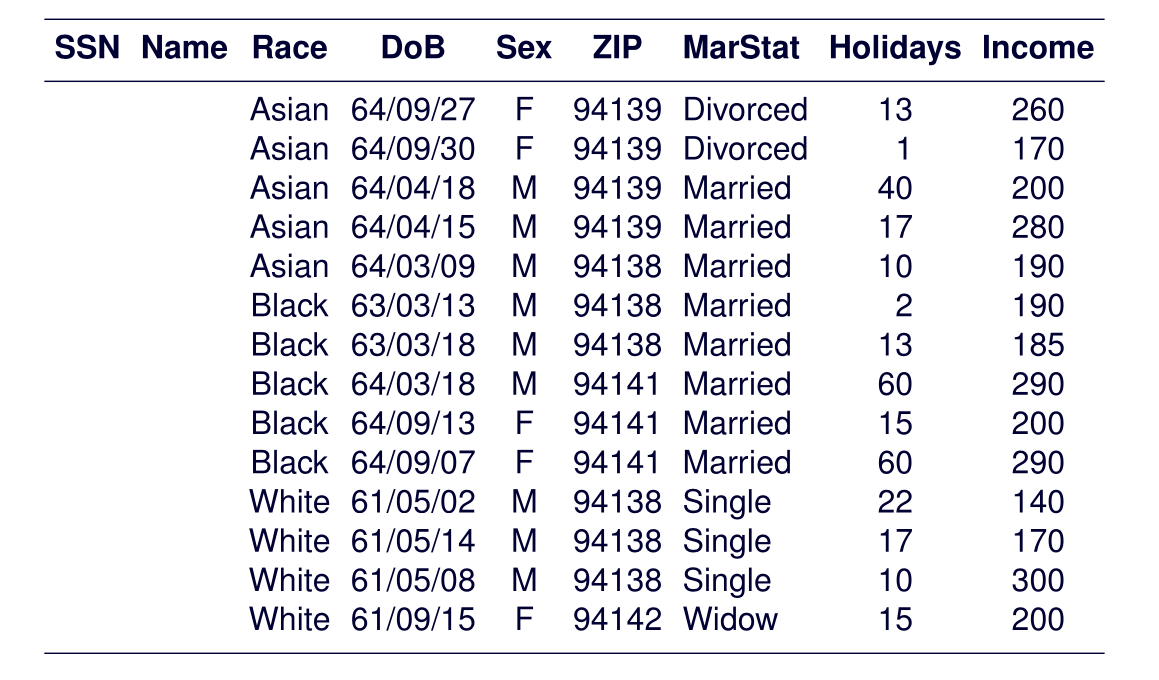
\includegraphics[width=1\linewidth]{images/base-ex.png}
\end{figure}

\subsection{Sampling [NP]}
La tabella protetta viene ottenuta facendo un campione della tabella di microdata 
originale. Viene introdotta dell'incertezza riguardo alla partecipazione di un 
rispondente, dunque diminuisce il rischio di reidentificazione.

\begin{figure}[ht]
    \centering
    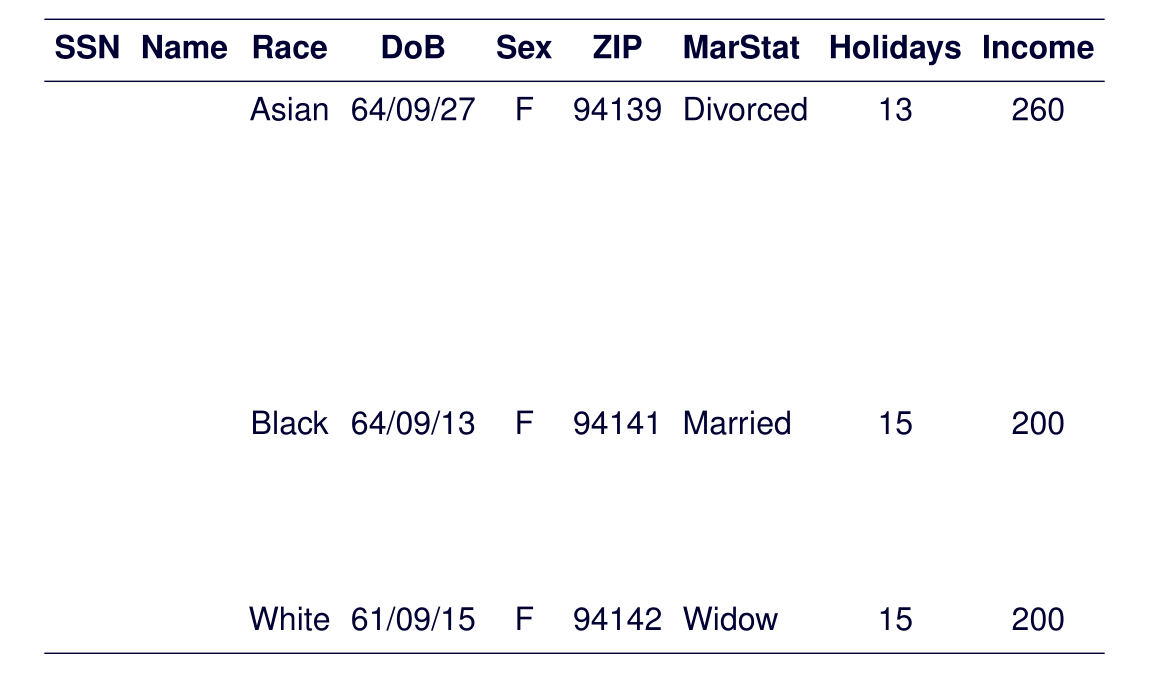
\includegraphics[width=0.75\linewidth]{images/sampling.png}
\end{figure}

\subsection{Local Suppression [NP]}
Sopprime il valore di un attributo che potrebbe contribuire in modo 
significativo al rischio di divulgazione, limitando le possibilità
di analisi.

\begin{figure}[ht]
    \centering
    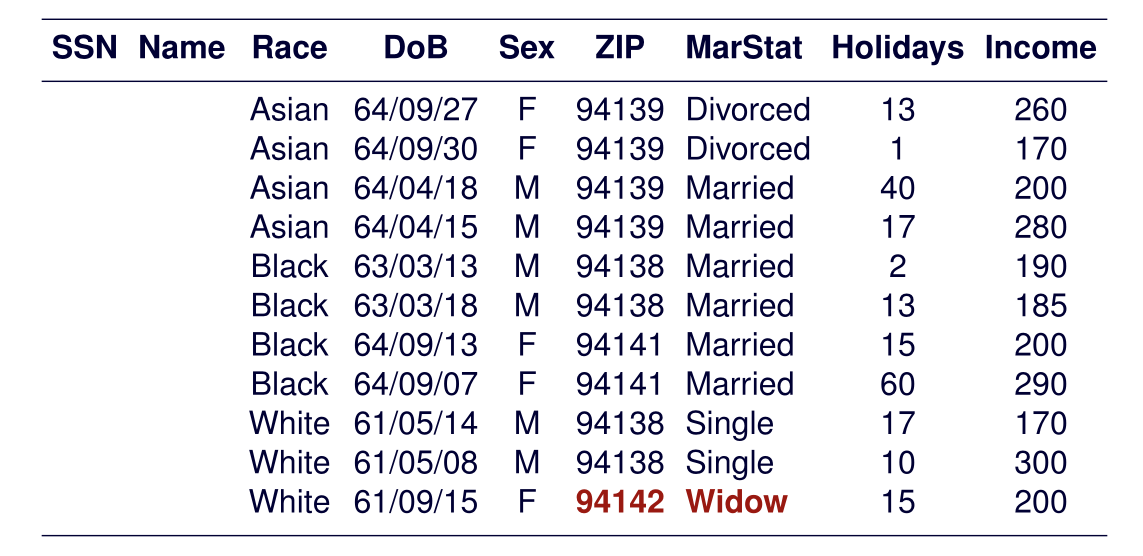
\includegraphics[width=0.75\linewidth]{images/local-sup.png}
\end{figure}

\subsection{Global Recoding [NP]}
Comporta la suddivisione del dominio di un attributo in diversi
intervalli disgiunti, tipicamente della stessa ampiezza, dove per 
ogni intervallo viene associata una \textit{label}.

La tabella protetta è ottenuta sostituendo i valori dell'attributo
con la \textit{label} associata all'intervallo corrispondente.

\begin{figure}[ht]
    \centering
    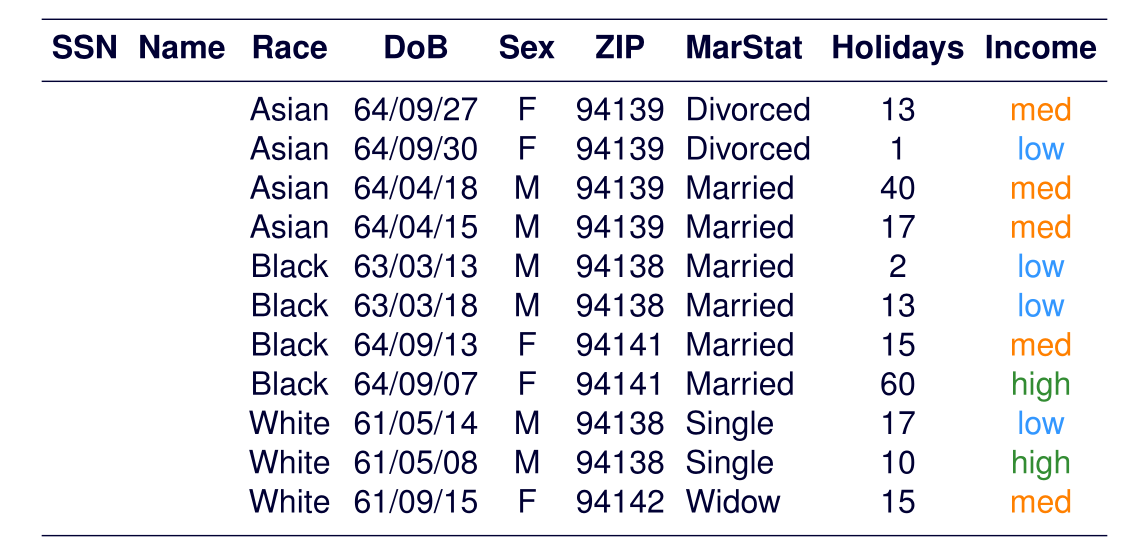
\includegraphics[width=0.75\linewidth]{images/global-recoding.png}
\end{figure}

\subsection{Top-coding e Bottom-coding [NP]}
Il \textit{top-coding} stabilisce un limite superiore per ciascun attributo 
da proteggere; qualsiasi valore maggiore di tale limite viene sostituito con 
una \textit{flag} che indica all'utente che tale valore supera il limite.

La procedura è ananloga per il \textit{bottom-coding} rispetto a un limite inferiore.

\begin{figure}[ht]
    \centering
    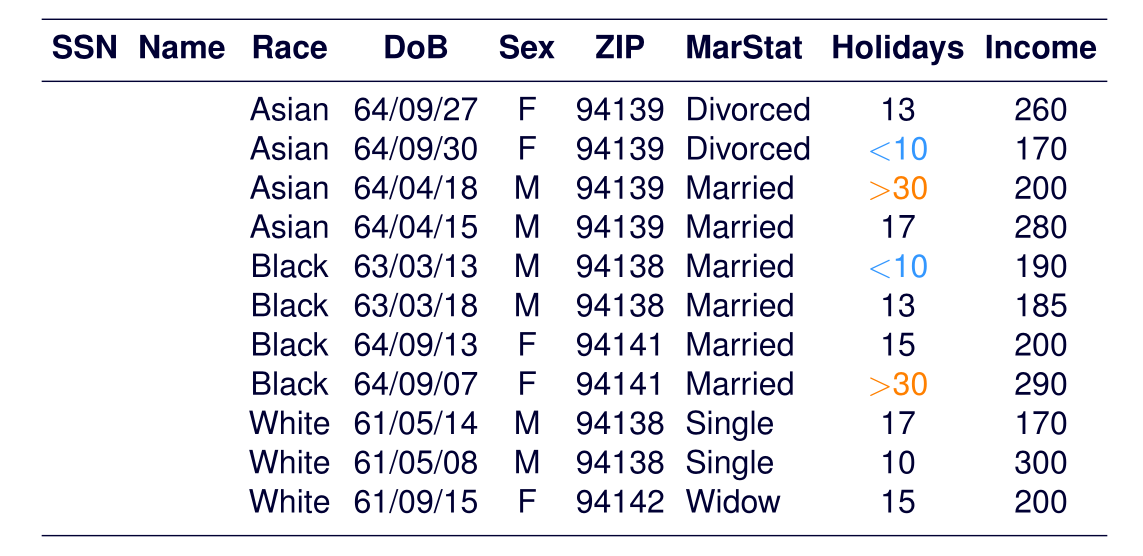
\includegraphics[width=0.75\linewidth]{images/top-bottom.png}
\end{figure}

\subsection{Generalizzazione [NP]}
I valori vengono sostituiti con altri più generali. È basata 
sulla definizione di una gerarchia di generalizzazione.

\begin{figure}[ht]
    \centering
    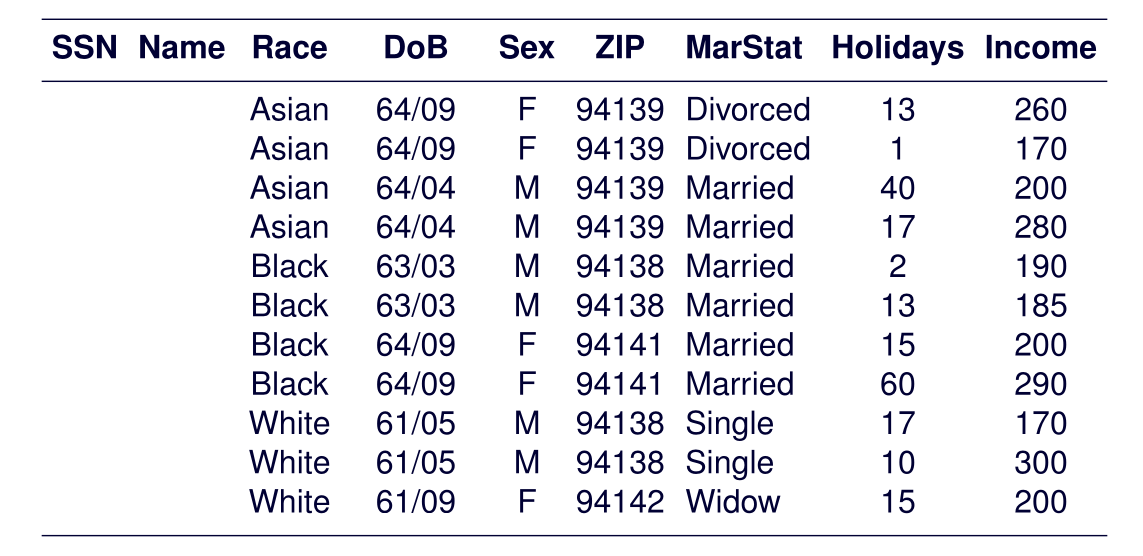
\includegraphics[width=0.75\linewidth]{images/gener.png}
\end{figure}

\subsection{Rumore casuale [P]}
Il rumore casuale perturba un attributo sensibile aggiungendo o moltiplicando 
il suo valore con una variabile casuale di una distribuzione specificata.

È necessario decidere se pubblicare o meno la distribuzione usata per aggiugere rumore ai dati;
la pubblicazione potrebbe aumentare il rischio di disclosure.

La somma del rumore introdotto deve essere pari a 0 per preservare la statistica.

\begin{figure}[ht]
    \centering
    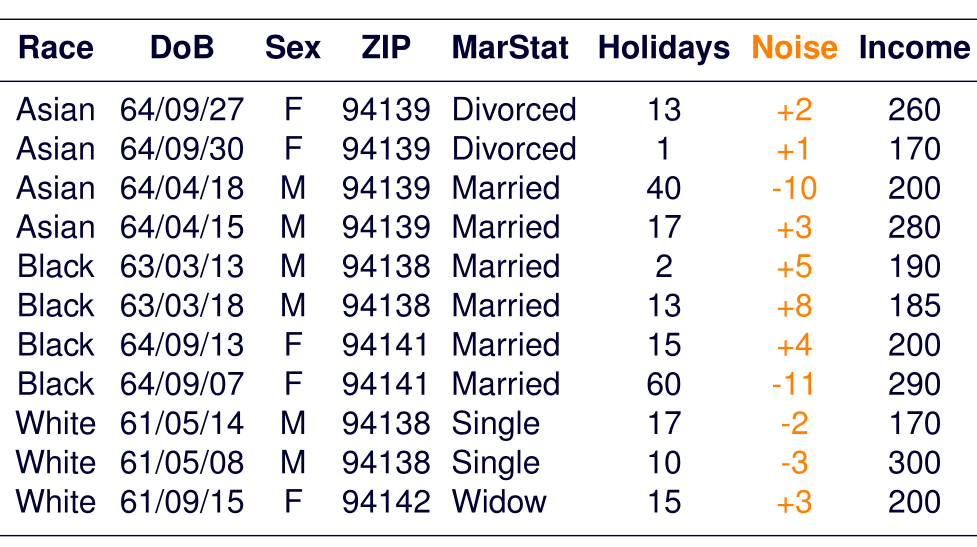
\includegraphics[width=0.75\linewidth]{images/noise1.png}
\end{figure}
\begin{figure}[ht]
    \centering
    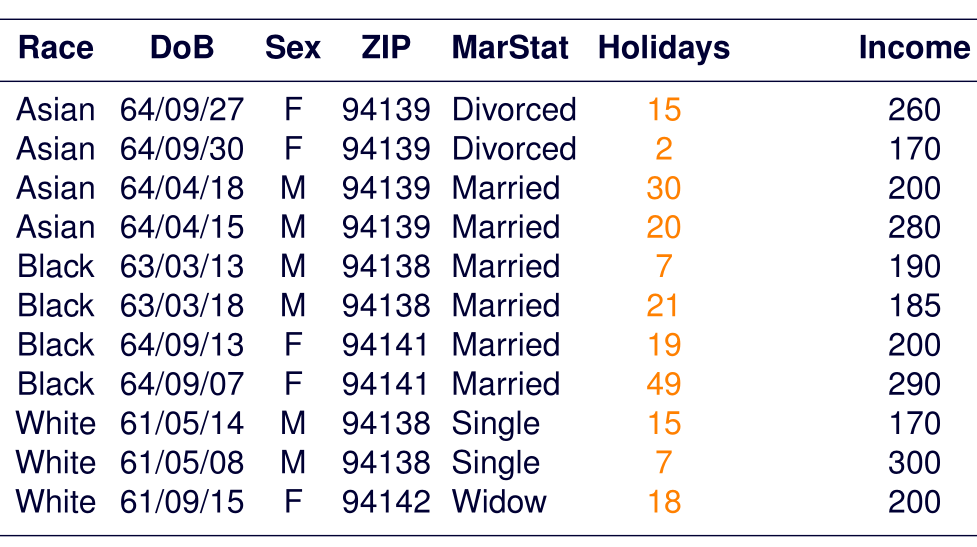
\includegraphics[width=0.75\linewidth]{images/noise2.png}
\end{figure}

\newpage
\subsection{Swapping [P]}
\subsubsection{Spiegazione con esempio}
Alcuni record potrebbero \textit{matchare} con altri record dello stesso 
file su alcuni attributi prefissati, ma appartenere a diverse zone geografiche.

I valori di tutte le altre variabili vengono scambiati. Questa tecnica 
riduce il rischio di reidentificazione dato che introduce incertezza
sulla veridicità del dato di un rispondente.

\begin{figure}[ht]
    \centering
    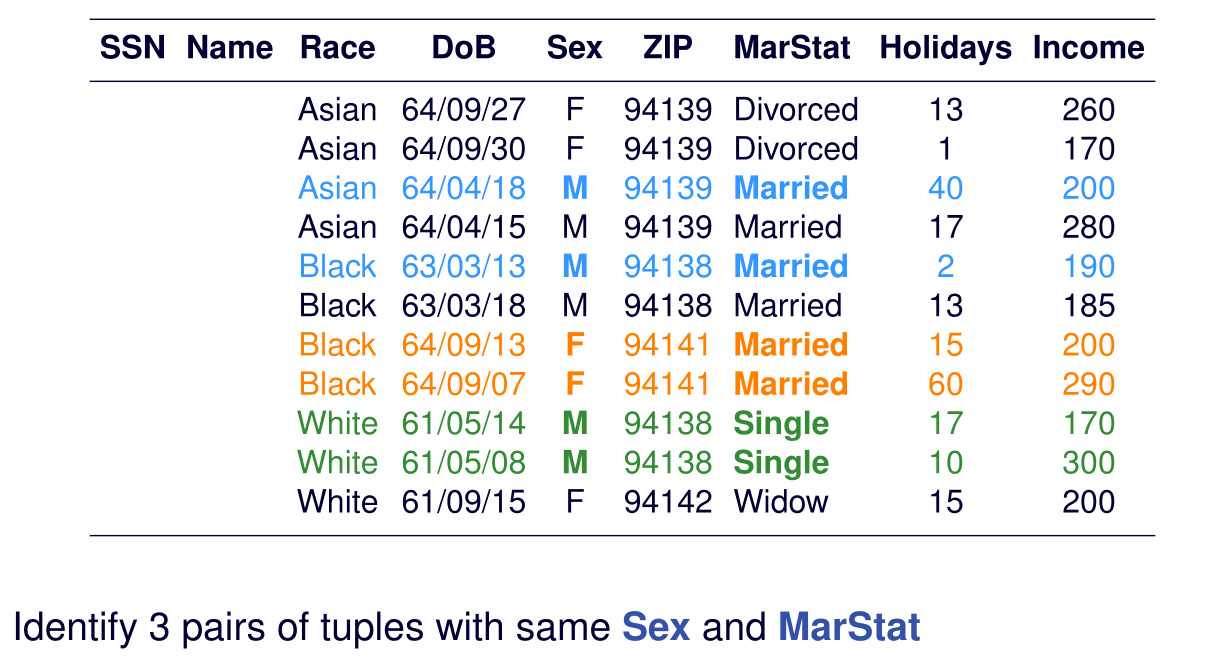
\includegraphics[width=0.75\linewidth]{images/swapping1.png}
\end{figure}
\begin{figure}[ht]
    \centering
    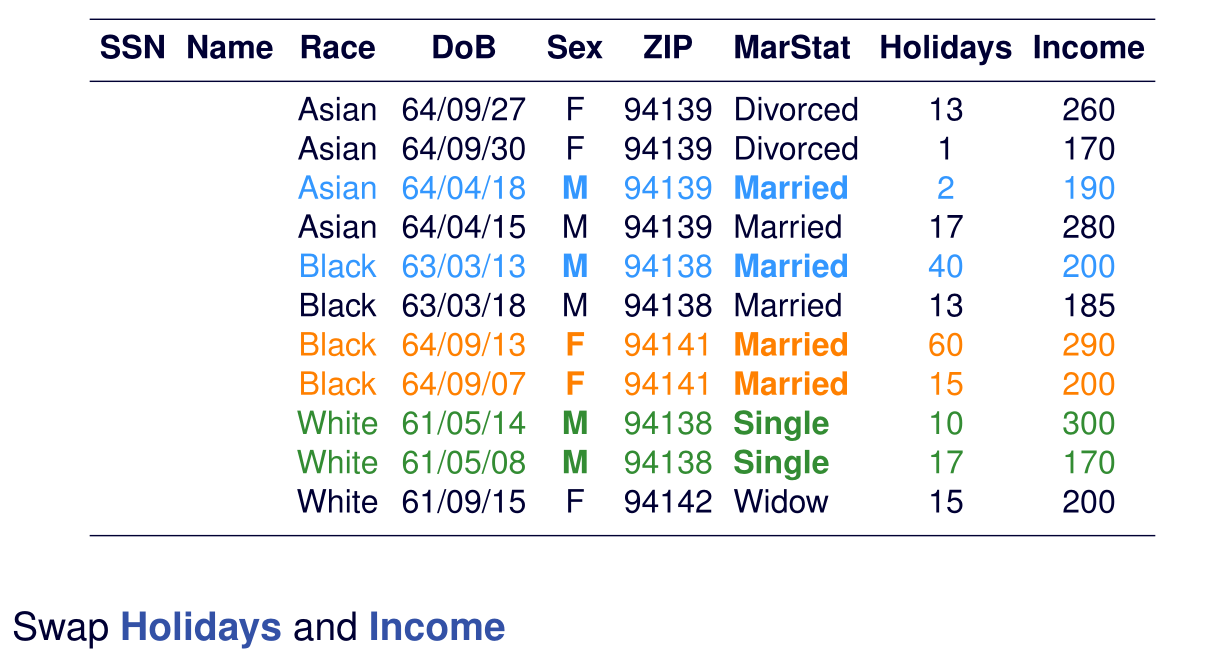
\includegraphics[width=0.75\linewidth]{images/swapping2.png}
\end{figure}

\newpage
\subsection{Micro-aggregation [P]}
La micro-aggregazione consiste nel raggruppare più tuple in dei gruppi 
di dimensione $k$. Viene poi pubblicata la media di tale gruppo al posto 
dei singoli valori.

I gruppi sono formati usando critieri di massima similarità.

\begin{figure}[ht]
    \centering
    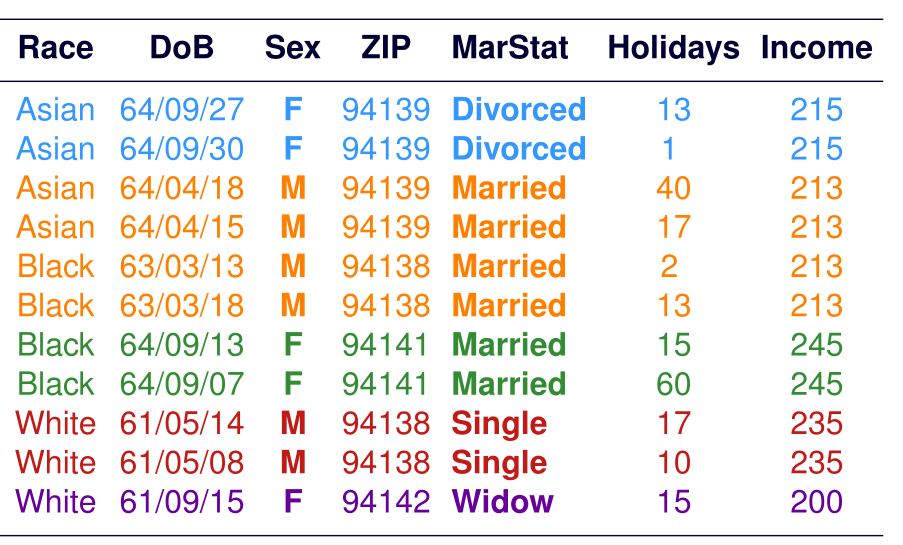
\includegraphics[width=0.75\linewidth]{images/micro-agg.png}
\end{figure}

\newpage
\section{Tecniche Sintetiche}
Consistono nel generare dati sintetici per sostituire quelli dei rispondenti, 
in modo che venga mantenuta la correlazione statistica.

Il vantaggio nell'utilizzo di queste tecniche è che i dati sintetici
rilasciati non sono riferiti a nessun rispondente e il loro rilascio 
non può portare a reidentificazione.



\end{document}